
\section[Main Functions]{Main Functions}
\label{sec:main_functions}
\addcontentsline{toc}{section}{\thesection. Main Functions}

The \pkg{cubfits} package is composed of three main functions:
\begin{enumerate}
\item \code{cubfits()} fits models for sequences with observed $\phi$ 
      (expression level) values and measurement errors,
\item \code{cubappr()} approximates models for sequences without any observed
      $\phi$ values, and
\item \code{cubpred()} fits models for sequences with observed $\phi$ values
      and measurement errors, and then predicts $\phi$ values for sequences
      without observations.
\end{enumerate}
See package's help pages for details of other input options.\footnote{
\code{?cubfits::cubfits}, \code{?cubfits::cubappr}, and
\code{?cubfits::cubpred}.
}


\subsection[Demonstrations]{Demonstrations}
\label{sec:demonstrtions}
\addcontentsline{toc}{subsection}{\thesubsection. Demonstrations}

The \pkg{cubfits} package provides quick examples for its three main functions:
\begin{Code}
> demo(roc.train, 'cubfits')    # for cubfits()
> demo(roc.appr, 'cubfits')     # for cubappr()
> demo(roc.pred, 'cubfits')     # for cubpred()
\end{Code}
These \pkg{cubfits} demos perform short MCMC runs
and analyze toy datasets (\code{ex.train} and \code{ex.test}) for the
Ribosome Overhead Cost (ROC)~\citep{Shah2011}
which is shown in Figure~\ref{fig:plotbin}. The toy datasets have only 100
short sequences, and only 3 amino acids are considered.

For a standard data analysis, the process essentially consists of:
\begin{enumerate}
\item reading sequences and expressions files,
\item converting to appropriate data structures,
\item running a main function (MCMC),
\item summarizing MCMC outputs, and
\item plotting predictions.
\end{enumerate}
The \pkg{cubfits} package also provides an example using simulated data:
\begin{Code}
> demo(simu.roc, 'cubfits')     # cubfits() is called.
\end{Code}
Note that this demo will generate a fake sequence file (\code{toy_roc.fasta})
in FASTA format in the working directory, and (for testing)
read it back. Also, it converts the data into the correct format
needed by \code{cubfits()}, and finally runs MCMC and generates a plot.


\subsection[Modeling ROC]{Modeling ROC}
\label{sec:roc_model}
\addcontentsline{toc}{subsection}{\thesubsection. Modeling ROC}

\pkg{cubfits}~\citep{Chen2014cubfitspackage} utilizes a
Bayesian hierarchical model for codon useage bias
(CUB)~\citep{Gilchrist2007,Shah2011,Wallace2013,Gilchrist2014}.
The CUB model for ROC is
\begin{eqnarray}
\vec{y}_{ga} &
    \sim & Multinom(n_{ga}, \vec{p}_{a}),
    \label{eqn:glm} \\
\vec{p}_{a} & = &
    mlogit^{-1}(\log(\vec{\mu}_{a}) + \vec{\Delta_t}_{a} \phi_g),
    \label{eqn:link_fcn} \\
\log(\phi_{g, obs}) & \sim &
    N(\log(\phi_g) + \log(K_{bias}), \sigma^2_{obs}),  \mbox{ and }
    \label{eqn:prior_lv1} \\
\log(\phi_g) & \sim &
    N(-\sigma^2_{\phi}/2, \sigma^2_{\phi}).
    \label{eqn:prior_lv2}
\end{eqnarray}
Given gene $g$ and amino acid $a$,
$\vec{y}_{ga}$ is synonymous codon counts
following a multinomial distribution with parameters
$n_{ga}$ for total codons and $\vec{p}_{a}$ for probability of
synonymous codons.
The $mlogit^{-1}$ is an inversed multivariate logit
function of $\vec{\mu}_{a}$ mutation rate and $\vec{\Delta_t}_{a}$
elongation time. $\phi_g$ is protein production rate 
and $\phi_{g,obs}$ is observed expression.
$K_{bias}$ and $\sigma^2_{obs}$ are measurement bias and
error, respectively. $\sigma^2_{\phi}$ is dispersion of $\log(\phi_g)$.
We assume independence of amino acids and independence of genes, and both
contribute information to the CUB model.

The package implements MCMC algorithms of CUB model in three main functions.
\code{cubfits()} estimate model parameters for sequence with $\phi_{g,obs}$
and implements Equations~(\ref{eqn:glm}) to~(\ref{eqn:prior_lv2}).
\code{cubappr()} predicts expression for sequences without $\phi_{g,obs}$
that skips Equations~(\ref{eqn:prior_lv1}).
\code{cubpred()} estimates parameters for sequences with $\phi_{g,obs}$
and predicts expression for sequences without $\phi_{g,obs}$.
All functions can take options set by global objects such as
MCMC conditions and auxiliary control variables

Figure~\ref{fig:bayesian_model} displays dependence of the model.
The extended Bayesian hierarchical model with measurement errors
for predicting protein synthesis rates ``with'' or ``without''
gene expression ($\phi$) is abstracted in the dependence graph:
\begin{itemize}
\item
data hierarchy is in blue boxes,
\item
observed sequences are in a green solid circle, 
\item
gene expressions (may be ignored) are in a green dashed circle,
\item
unknown parameters to be estimated are in red dashed circles,
\item
prior parameters (may be restricted) are in the black circle, and
\item
parallelization within MCMC is in red dashed lines.
\end{itemize}
\begin{figure}[ht]
\centering
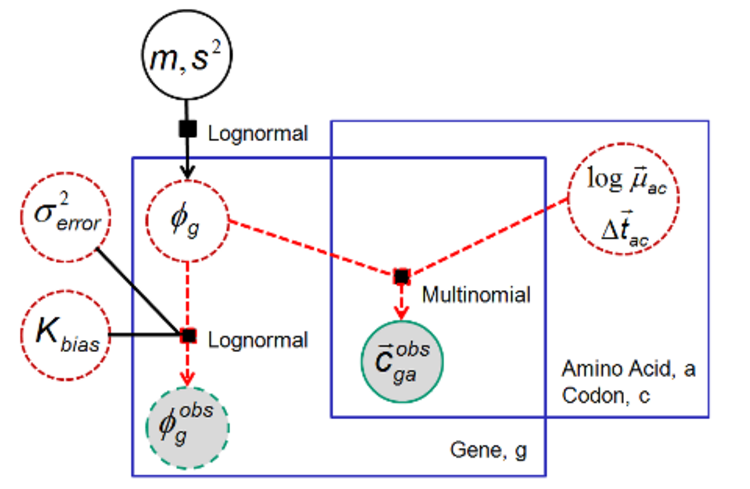
\includegraphics[width=5.5in]{cubfits-include/figure/bayesian_model}
\caption{Dependence plot of ROC model (after \citep{Wallace2013}).}
\label{fig:bayesian_model}
\end{figure}



\subsection[Generic Functions]{Generic Functions}
\label{sec:generic_functions}
\addcontentsline{toc}{subsection}{\thesubsection. Generic Functions}

Note that the three main functions are wrappers of other generic functions that
perform parameter initializations, propose new parameters, compute
MCMC acceptance/rejection ratio, and more.
The function \code{init.function()} initializes generic functions that
will be called by the three main functions.
Although \code{init.function()} is called within each of three main
functions to setup the generic functions, it also needs to be called before
using other utility functions, such as \code{fitMultinom()}, see
Section~\ref{sec:misc} for examples.

Accompanying control variables such as \code{.CF.CT} and \code{.CF.OP},
the \code{init.function()} will dispatch the
corresponding generic functions into a default environment \code{.cubfitsEnv},
allowing other main functions may call those generic functions dynamically.

Note that generic functions in \proglang{R} typically only depend on
input object types.  However, the design in \pkg{cubfits} has 
several advantages:
\begin{itemize}
\item functions are clearer by making good use of data structures and
      simplifying options,
\item extensions are easier to create; simply add more generic functions 
      rather than changing main functions, and
\item performance is more efficient by avoiding extra
      conditional checks such as \code{if(...)\{...\} else\{...\}}
      in every iteration.
\end{itemize}
Also, the design can avoid tedious CRAN checks since there are some restrictions
in accessing \code{.GlobalEnv}. For example, 
\code{.cubfitsEnv$my.fitMultinomAll()} is called in several
internal functions to fit multinomial logistic regression in every MCMC
iterations. In particular, it has four generic functions:
\begin{enumerate}
\item \code{my.fitMultinomAll.lapply()} ueses \code{lapply()} in the serial version,
\item \code{my.fitMultinomAll.mclapply()} uses \code{parallel::mclapply()}
      in shared memory machines,
\item \code{my.fitMultinomAll.task.pull()} uses \code{pbdMPI::task.pull()}
      in distributed clusters, and
\item \code{my.fitMultinomAll.pbdLapply()} uses \code{pbdMPI::pbdLapply()}
      in distributed clusters, but is only efficient for homogeneous tasks.
\end{enumerate}
Through \code{init.function()}, there is no need to check which generic
function should be called within the MCMC step, and there is no need to worry
about serial or parallel details when designing a MCMC algorithm.

